\documentclass{article}
\usepackage{graphicx} % Required for inserting images
\usepackage[english]{babel}
\usepackage{amsmath}
\usepackage{amsfonts}
\usepackage{amsthm}
\usepackage{amssymb}
\usepackage{physics}
\usepackage[mathscr]{euscript}
\let\euscr\mathscr \let\mathscr\relax
\usepackage[scr]{rsfso}
\newcommand{\powerset}{\raisebox{.15\baselineskip}{\Large\ensuremath{\wp}}}

\usepackage{mathtools}


\numberwithin{equation}{section}

\newcommand{\Set}[1]{\{#1\}}
\newcommand{\FT}{\mathcal{F}}
\newcommand\perm[2][^n]{\prescript{#1\mkern-2.5mu}{}P_{#2}}
\newcommand\comb[2][^n]{\prescript{#1\mkern-0.5mu}{}C_{#2}}

\DeclareMathOperator{\spn}{span}

\makeatletter
\renewcommand*\env@matrix[1][*\c@MaxMatrixCols c]{%
  \hskip -\arraycolsep
  \let\@ifnextchar\new@ifnextchar
  \array{#1}}
\makeatother

\newtheorem{theorem}{Theorem}[section]
\newtheorem{corollary}{Corollary}[theorem]
\newtheorem{lemma}[theorem]{Lemma}
\title{PHYS100A Homework 10}
\author{Siyu Chen}
\date{July 2023}

\begin{document}

\maketitle

\section{Section 9, page 582: problem 9}
Expand the following functions in Legendre series.
\begin{align*}
    f(x) = P'_n(x)
\end{align*}

Since the coefficients of our Legendre series, from previous derived results (in Homework 9, part c), can be written as the following

\begin{align}
    c_m  = \frac{2m+1}{2} \int_{-1}^{1} f(x) P_m(x)dx
\end{align}

now, substitute in our defined function, we can see that (1.1) is expressed as:

\begin{align}
    c_m = \frac{2m+1}{2} \int_{-1}^{1} P'_n(x) P_m(x)dx
\end{align}

We can notice that as long as $m \geq n$, the integral should return $0$. This is because if $P_m$ is a polynomial of degree $m$, then at most in the case that $n = m$, $P_n$ is a polynomial of degree $m$ as well, then $P'_n$ is a polynomial of degree $m-1$, so in general, the degree of $P_n$ is less than or equal to $m-1$. Now, because Legendre polynomials are orthonormal, for the space of polynomials of degree $m-1$, the set of Legendre polynomials with degree less than or equal to $m-1$ form a basis for that space, or 
\begin{align}
    \spn \Set{ P_l(x) : 0 \leq l \leq m-1 } = \mathscr{P}_{m-1} (x)
\end{align}

Since $P'_n \in \mathscr{P}_{m-1}$, we can write it as a linear combinations of Legendre polynomials of the set that we just described, i.e

\begin{align}
    P'_n(x) = a_1 P_1(x) + \ldots a_{n-1} P_{n-1}(x)
\end{align}

Therefore the integral in (1.2) can be written as

\begin{align}
    a_1 \int_{-1}^{1} P_1(x) P_m(x)dx + \ldots + a_{n-1} \int_{-1}^{1} P_{n-1} P_m(x)dx
\end{align}

and since Legendre polynomials are orthogonal, our integrals are, of course, 0, and (1.2) must return $0$ for $n \leq m$. This means that $c_m = 0$ for $m \geq n$ For the case of $n > m$, integrating our integral by parts, we obtain

\begin{align}
    \int_{-1}^{1} P'_n(x) P_m(x) dx = P_n(x) P_m (x) - \int_{-1}^{1} P_n(x) P'_m(x) dx
\end{align}

Since in this case, $n > m$, and by the same logic that the inner product between a Legendre polynomiad and any polynomial of lesser degree is $0$, we have 

\begin{align}
    \int_{-1}^{1} P'_n(x) P_m(x) dx = P_n(x) P_m (x), \quad n > m
\end{align}

Finally, using (1.2) to compute our constants, we have:

\begin{align}
    c_m = \begin{cases}
        \frac{2m+1}{2} P_n(x) P_m(x) \quad &m < n \\
        0, &m \geq n
    \end{cases}
\end{align}

\section{Section 2, page 626: problem 2}
Solve the semi-infinite plate problem if the bottom edge of width 20 is held at 
\begin{align*}
    T(x,y) = \begin{cases}
        0^{\circ}, \quad &0 < x < 10, \\
        100^{\circ}, \quad &10 < x < 20
    \end{cases}
\end{align*}

and the other sides are at $0^{\circ}$

Assume that $y$ extends to infinity. We are solving the 2-D Laplace's Equation of 

\begin{align}
    \grad^2 T(x,y) = 0
\end{align}

Using separation of variables, let 

\begin{align}
    T(x,y) = X(x) Y(y)
\end{align}

and (3.1) as a result becomes:

\begin{align}
    Y \frac{\partial^2 X}{ \partial x^2} + X \frac{\partial^2 Y}{\partial y^2} = 0
\end{align}

and re-arranging, we have:

\begin{align}
    \frac{1}{X} \frac{\partial^2 X}{ \partial x^2} = - \frac{1}{Y} \frac{\partial^2 Y}{\partial y^2} = -k^2
\end{align}

we can identify the differential equation for $X, Y$ respectively. We have:

\begin{align}
    X'' + k^2 X = 0, \quad Y'' - k^2 Y = 0
\end{align}

The set of solutions for them are:

\begin{align}
    X = \spn\Set{ \sin kx, \cos kx}, \quad Y = \spn\Set{e^{ky}, e^{-ky}}
\end{align}

and $T$ is the product of the two sets. Consider our boundary conditions, first, since $\lim_{y\to \infty} T(x,y) = 0$ as the top side of the plate is at temperature $0^\circ$. We can discard any solution of $e^{ky}$ since $\lim_{y\to \infty} e^{ky} \neq 0$. Then, our solution is of the form:

\begin{align}
    T(x,y) = a e^{-ky} (b \sin kx + c\cos kx)
\end{align}

If $y > 0, x = 0 \vee x = 20, T = 0 ^\circ$ as the other sides start with temperatures of $0^\circ$, we have

\begin{align}
    T(0, y) &= 0, T(20, y) = 0^\circ \\
    T(0, y) &= a e^{-ky} (c \cos kx) = 0^\circ
\end{align}

This means that since $a e^{-ky}, \cos kx$ is not 0 in general, then it is necessary that $c = 0$ and we discard the cosine term as well. Our general solution is now

\begin{align}
    T(x,y) = A e^{-ky} \sin kx
\end{align}

Where $A = ab$ from our previous temporarily defined constants. At $y = 0$, we have 

\begin{align}
    T(x,0) &= A \sin kx, \\
    T(x,0) &= \begin{cases}
        0^{\circ}, \quad &0 < x < 10, \\
        100^{\circ}, \quad &10 < x < 20 \\
        0^{\circ}, \quad &x = 0, x = 20
    \end{cases}
\end{align}

where (2.10) is from our solutions, and (2.11) is from our boundary conditions. Using just the third line of (2.11), which we obtain from the sides being $0^\circ$, our solution must be of the form

\begin{align}
    T(x,0) = A \sin{\frac{n \pi x}{20}} 
\end{align}

This becomes a Fourier Series problem with our last boundary condition. Evaluating the coefficient, we have 

\begin{align}
    b_n = \frac{1}{20}\int_{0}^{20} f(x) \sin \frac{n \pi x}{20} = \frac{1}{20} \int_{10}^{20}100 \sin \frac{n \pi x}{20} = \frac{200}{\pi n} (\cos(\frac{\pi n}{2}) - \cos(\pi n))
\end{align}

Thus (2.10) becomes:

\begin{align}
    T(x,y) = \frac{200}{\pi}\sum_{n=}^{\infty} \frac{1}{n}(\cos(\frac{\pi n}{2}) - \cos(\pi n)) e^{-\frac{n\pi y}{20}} \sin \frac{n\pi x}{20}
\end{align}

Wolfram Alpha gives the following plot at $n=100$

\begin{figure}[!htb]
   \begin{minipage}{0.48\textwidth}
     \centering
     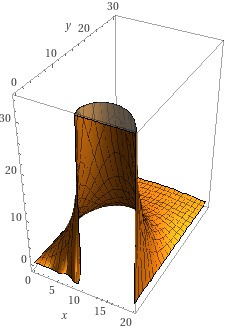
\includegraphics[width=.7\linewidth]{plot2.1.jpg}
     \caption{3-D map of $T(x,y)$}\label{Fig: 2.1}
   \end{minipage}\hfill
   \begin{minipage}{0.48\textwidth}
     \centering
     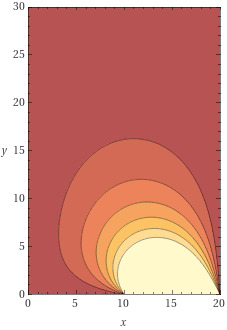
\includegraphics[width=.7\linewidth]{plot2.2.jpg}
     \caption{Contour map of $T(x,y)$}\label{Fig: 2.2}
   \end{minipage}
\end{figure}

We can see that this makes sense since our solution allows heat to diffuse off the high temperature line of $10<x<20$, and spread heat to rest of the region.

\section{Section 3, page 632: problem 4}

At t = 0, two flat slabs each 5 cm thick, one at $0^\circ$ and one at $20^\circ$, are stacked together, and then the surfaces are kept at $0^\circ$. Find the temperature as a function of $x$ and $t$ for $t > 0$.

Our initial conditions for our $u(x,t)$ are:

\begin{align}
    u(0, t) &= u(20, t) = 0^\circ \\
    u(x, 0) &= 20^\circ \quad 0 < 5 < 10
\end{align}

Since our system only concerns the $x$-direction, we can use the diffusion heat equation:

\begin{align}
    \frac{\partial^2 u}{\partial x} = \frac{1}{\alpha^2} \frac{\partial u}{\partial t}
\end{align}

now using separation of variables:

\begin{align}
    u(x,t) = X(x)T(t)
\end{align}

and our equation becomes:

\begin{align}
    T(t) \frac{\partial^2 X}{\partial x^2} = \frac{1}{\alpha^2} X(x) \frac{\partial T}{\partial t} 
\end{align}

rearranging and equating each side to constant, we have:

\begin{align}
    \frac{1}{X(x)} \frac{\partial^2 u}{\partial x^2} = \frac{1}{\alpha^2} \frac{1}{T(t)} \frac{\partial T}{\partial t} = -k^2
\end{align}

solving for each differential equations, we can obtain the following: 

\begin{align}
    T(t) = t_0 e^{-k^2 \alpha^2 t} \quad X(x) = x_1 \cos(kx) + x_2 \sin(kx)
\end{align}

Now, to satisfy our boundary condition, we can see that since at $x = 0, u = 0$ from our boundary condition, we can discard our $\cos(kx)$ term as $\cos(0) = 1$. We then can write our solution in the form of:

\begin{align}
    u(x,t) = A \sin(kx) e^{-k^2 \alpha^2 t}
\end{align}

where $A$ is a constant. Now to satisfy our initial conditions, we have:

\begin{align}
    u(x,0) = A \sin(kx) = \begin{cases}
        20^\circ \quad &(0<x<5) \\
        0^\circ \quad &(5<x<10)
    \end{cases} 
\end{align}

This is a Fourier Series problem and from our boundary condition, our solution must be in the form of:

\begin{align}
    u(x,0) = \sum_{n=0}^{\infty} b_n \sin \frac{n \pi x}{10} 
\end{align}

Evaluating for our constants, we have:

\begin{align}
    b_n = \frac{1}{10}\int_{0}^{10} f(x) \sin \frac{n \pi x}{10} = 2 \int_{5}^{10} \sin \frac{n\pi x}{10} = \frac{40}{\pi n} ( \cos(\frac{\pi n}{2}) - \cos(\pi n))
\end{align}

we can then write our solution in terms of a series as:

\begin{align}
    u(x,t) = \frac{40}{\pi} \sum_{n=1}^{\infty} \frac{1}{n} ( \cos(\frac{\pi n}{2}) - \cos(\pi n)) \sin \frac{n\pi x}{10} e^{-\alpha^2 \frac{n^2\pi^2}{100}t}
\end{align}

Wolfram Alpha gives the following graphs for $n=100, \alpha = 1$

\begin{figure}[!htb]
   \begin{minipage}{0.48\textwidth}
     \centering
     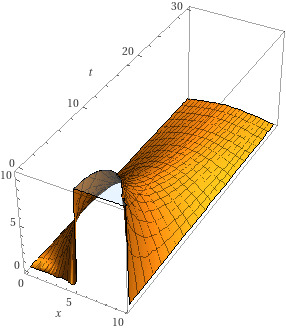
\includegraphics[width=.7\linewidth]{plot3.1.jpg}
     \caption{3-D map of $u(x,t)$}\label{Fig: 3.1}
   \end{minipage}\hfill
   \begin{minipage}{0.48\textwidth}
     \centering
     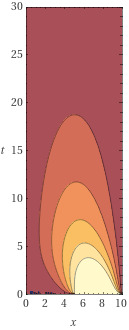
\includegraphics[width=.7\linewidth]{plot3.2.jpg}
     \caption{Contour map of $u(x,t)$}\label{Fig: 3.2}
   \end{minipage}
\end{figure}

We can see that this graph makes sense as, without additional heat source, the high temperature slab begins to gradually lose its temperature over time to the environment kept at $0^\circ$ while conducting some heat to the adjacent slab.

\section{Section 7, page 650: problem 4}

Find the steady-state temperature distribution inside a sphere of radius 1 when the surface temperatures are

\begin{align*}
    T(1, \theta, \phi) = 5 \cos^3 \theta - 3 \sin^2 \theta
\end{align*}

The solution for a spherical Laplacian equation in this case (inside the sphere) is:

\begin{align}
    u(r, \theta, \phi) = \sum_{n=1}^{\infty} c_l r^l P_l(\cos \theta)
\end{align}

along with our initial boundary conditions, we have:

\begin{align}
    u(1, \theta, \phi) = \sum_{n=1}^{\infty} c_l P_l(\cos \theta) = 5 \cos^3 \theta + 3 \cos^2 \theta - 3
\end{align}

We can see that this is equal to

\begin{align}
    u(1, \theta, \phi) = 2 P_3(\cos\theta) + 2 P_2 (\cos \theta) + 3 P_1 (\cos\theta) -  P_0(\cos \theta)
\end{align}

Plugging back, our solution becomes:

\begin{align}
    u(r, \theta, \phi) = 2 r^3 P_3(\cos\theta) + 2 P_2 r^2 (\cos \theta) + 3 r P_1 (\cos\theta) -  P_0(\cos \theta)
\end{align}

(Note: we are taking the result from textbook as is for Laplacian inside a sphere. If we go from the general solution, we would discard the term $r^{-l-1}$ due to it diverging at $r = 0$, and the $\phi$ terms must be 1 as $e^{im\phi}$ term not showing up in our initial boundary condition means that $m = 0$, so then we can use (4.1) directly to obtain our results.)




\end{document}
